\documentclass{article}
\usepackage[utf8]{inputenc}
\usepackage{amsmath,amsthm,amssymb,graphicx,mathtools,tikz,hyperref}
\usepackage[round]{natbib}
\usepackage{listings}
\usepackage{graphicx}
\graphicspath{ {../figures/} }

\title{Analytical approximation for LOO-R2 standard error}
\author{Leevi Lindgren \footnote{I thank Aki Vehtari and Nikolas Siccha for their comments.}}
\date{\today}

\begin{document}

\maketitle

\section{Introduction}
R-squared, or R2, is a typical measure used to assess how well a model fits data. \cite{gelman_r-squared_2019} propose a Bayesian version of the R2 as the classical R2 might get values larger than 1 for Bayesian regression models. See details from the paper. A nice property of Bayesian R2 is that we get a distribution of R2 values "for free", as it is computed using posterior predictive mean values of the model. This means that we can quantify the uncertainty of the estimator easily.

If (Bayesian) R2 is computed from the same data that was used to fit the model, it will give an overestimate of the predictive performance on a new, unobserved data. As often we don't have independent test data, we can use cross-validation to estimate the out-of-sample behavior of the R2. \cite{vehtari_practical_2016} propose an efficient and stable method for leave-one-out cross-validation using Pareto smoothed importance sampling. In the paper, log predictive density is used as the utility describing the predictive performance, but the method can easily be extended for other utilities as well, such as R2.

After computing LOO-R2 estimate, we obviously want to quantify the uncertainty of the estimator. The uncertainty in LOO-R2 comes from not knowing the future data distribution \citep{vehtari_survey_2012}. One way to do it is to use Bayesian bootstrap \citep{rubin_bayesian_1981}. However, this report describes how to quantify the uncertainty using an analytical Taylor approximation approach.

The idea is to note that LOO-R2 is defined as a function of a ratio of two random variables. We can then use Taylor approximation of the function and the mean, variance, and covariance of the two random variables to approximate the standard error of the LOO-R2 estimator. 

This approach was motivated by the work by \cite{hastings1970monte} who proposes an approximation for the variance of the ratio of two random variables. However, the formula provided by cite{hastings1970monte} contains two typos: on page 8, in the formula for the variance of the ratio, $Z$ is missing the "bar" symbol and computed variance $s_{\bar{Z}}$ is missing the second power. The missing second power caused the author of this report to mistake it for the standard deviation instead of variance, which was followed by weird simulation results. 

\section{Taylor approximation for a function of two variables}

Let $f(x, y): \mathbb{R}^2 \rightarrow \mathbb{R}$ be a function of two (random) variables. The first order Taylor approximation of a function of two variables around point $x_0, y_0$ is given by
\begin{align}
    f(x, y) &\approx f(x_0, y_0) + \frac{\partial }{\partial x} f(x_0, y_0) (x - x_0) + \frac{\partial }{\partial y} f(x_0, y_0) (y - y_0) \label{tapprox}
\end{align}

Now, let's take two random variables $X$ and $Y$ and do the approximation around the expected values $(\mu_X, \mu_Y)$ = $(E[X], E[Y])$. Using \eqref{tapprox} we get
\begin{align}
    f(X, Y) \approx f(\mu_X, \mu_Y) + \frac{\partial }{\partial x} f(\mu_X, \mu_Y) (X - \mu_X) + \frac{\partial }{\partial y} f(\mu_X, \mu_Y) (Y - \mu_Y) \label{rvtapprox}
\end{align}

\subsection{Taylor approximation for the expected value}
Given that terms containing partial derivatives in \eqref{rvtapprox} go to zero under expectation, we get the following, simple, first order approximation for the expected value of $f(X, Y)$:
\begin{align}
    E[f(X, Y)] \approx f(\mu_X, \mu_Y) \label{eapprox}
\end{align}

\subsection{Taylor approximation for variance}
For variance
\begin{align}
    \text{var}(f(X, Y)) &= E\left[ \left(f(X, Y) - E[f(X,Y)] \right)^2 \right] \nonumber \\
    &\approx E\left[ \left( f(X, Y) - f(\mu_X, \mu_Y) \right)^2 \right] \nonumber
\end{align}
Next, we plug in \eqref{rvtapprox} for $f(X,Y)$ which yields (we write $\frac{\partial }{\partial x} f(\mu_X, \mu_Y) = \frac{\partial f}{\partial x}$ for notational simplicity):
\begin{align}
    \text{var}(f(X, Y)) &\approx E\left[ \left( \frac{\partial f}{\partial x} (X - \mu_X) + \frac{\partial f}{\partial y} (Y - \mu_Y) \right)^2 \right] \nonumber \\
    &= E\left[ \left( \frac{\partial f}{\partial x}  \right)^2 (X - \mu_X)^2 + 2 \frac{\partial f}{\partial x} \frac{\partial f}{\partial y} (X - \mu_X)(Y - \mu_Y) + \left( \frac{\partial f}{\partial y}  \right)^2 (Y - \mu_Y)^2  \right] \nonumber \\
    &= \left( \frac{\partial f}{\partial x}  \right)^2 \text{var}(X) + 2 \frac{\partial f}{\partial x} \frac{\partial f}{\partial y} \text{cov}(X, Y) + \left( \frac{\partial f}{\partial y}  \right)^2 \text{var}(Y) \label{varapprox}
\end{align}

\section{Approximation for the standard error of LOO-R2}
LOO-R2 is defined as
\begin{align}
\text{R2}_{loo} = 1 - \frac{\text{var}(\hat{e}_{loo}) }{ \text{var}(y)} \label{loor2}
\end{align}

where $\hat{e}_{loo} = y - \hat{y}_{loo}$. Note that the nominator and denominator of the second term in \eqref{loor2} can be interpreted as the mean squared error of the LOO predictions and mean squared error of predicting the data with its mean, respectively. So we write \eqref{loor2} as 
\begin{align}
    \text{R2}_{loo} = 1 - \frac{\text{MSE}_{\hat{e}} }{ \text{MSE}_y} \label{mser2}
\end{align}

We can then compute the estimator for the variance of both using the same approach as in \cite{sivula_uncertainty_2022} and \cite{vehtari_practical_2016}:
\begin{align}
    \text{var}(\text{MSE}_{\hat{e}}) &= \frac{1}{n (n-1)} \sum_{i = 1}^n \left( \hat{e}_{loo, i}^2 - \text{MSE}_{\hat{e}} \right)^2 \label{vare}
\end{align}
and
\begin{align}
    \text{var}(\text{MSE}_y) &= \frac{1}{n (n-1)} \sum_{i = 1}^n \left( (y_i - \hat{y})^2 -\text{MSE}_y \right)^2 \label{vary},
\end{align}
where $\bar{y}$ is the sample mean of observations $y$. 

To utilize the Taylor approximation, we need to compute partial derivatives of function $f(x,y) = 1 - \frac{x}{y}$. With a simple calculus, we get
\begin{align}
    \frac{\partial}{\partial x}f(x,y) = -\frac{1}{y} \\
    \frac{\partial}{\partial y}f(x,y) = \frac{x}{y^2}.
\end{align}

Substituting these into \eqref{varapprox} yields
\begin{align}
    \text{var}(f(X, Y) \approx \frac{1}{\mu_Y^2} \left( \text{var}(X) - 2 \frac{\mu_X}{\mu_Y} \text{cov}(X,Y) + \left( \frac{\mu_X}{\mu_Y} \right)^2 \text{var}(Y) \right) \label{ratiovar}.
\end{align}

 To use this expression for the mean squared errors, we also need the covariance between $\text{MSE}_{\hat{e}}$ and $\text{MSE}_y$. This can be estimated in a similar way as the variances:
 \begin{align}
     \text{cov}(\text{MSE}_{\hat{e}}, \text{MSE}_{y} ) = \frac{1}{n (n -1 )} \sum_{i = 1}^n \left( \hat{e}_{loo, i}^2 - \text{MSE}_{\hat{e}} \right) \left( (y_i - \hat{y})^2 -\text{MSE}_y \right) \label{cov}.
 \end{align}
 
 Putting all pieces together, variance, and consequently the standard error, of LOO-R2 estimator can then be approximated by letting $\mu_X = \text{MSE}_{\hat{e}}$ and $\mu_Y = \text{MSE}_y$ and then substituting with \eqref{vare}, \eqref{vary} and \eqref{cov} into \eqref{ratiovar}:
 \begin{align}
     \text{var}(\text{R2}_{loo}) &= \frac{1}{\text{MSE}_y^2} \left( \text{var}(\text{MSE}_{\hat{e}}) - 2 \frac{\text{MSE}_{\hat{e}}}{\text{MSE}_y} \text{cov}(\text{MSE}_{\hat{e}}, \text{MSE}_{y} ) +  \left( \frac{\text{MSE}_{\hat{e}}}{\text{MSE}_y} \right)^2 \text{var}(\text{MSE}_y) \right) \label{estimator}.
 \end{align}
 
\section{Simulation experiments}
To illustrate behaviour of the proposed analytical approximation, we run a set of simulations with a few different configurations. We proceed as follows: choose number of observations $n$, number of predictors $p$ and observational noise $\sigma$ and then, draw predictor matrix $X \in \mathbb{R}^{n \times p}$ and $\beta \in \mathbb{R}^{p}$ from $N(0, 1)$ and  $\epsilon \in \mathbb{R}^{n}$ from $N(0, \sigma^2)$. Then we compute $y = X \beta + \epsilon$ for which we with linear model using R-package rstanarm \citep{rstanarm}. We repeat this for 100 for each set of parameters. See underlying code from \url{https://github.com/LeeviLindgren/loo-r2-se}.

Figure \ref{fig:simres} plots standard error obtained from the Taylor approximation and Bayesian bootstrap for different values of $n$, $\sigma$, and $p$. The diagonal line represents points where x and y-axis values are equal and the actual simulation results are represented with the dots. Dots' color indicates the underlying LOO-R2 estimate obtained by taking the mean of BB samples.
\begin{figure}
    \centering
    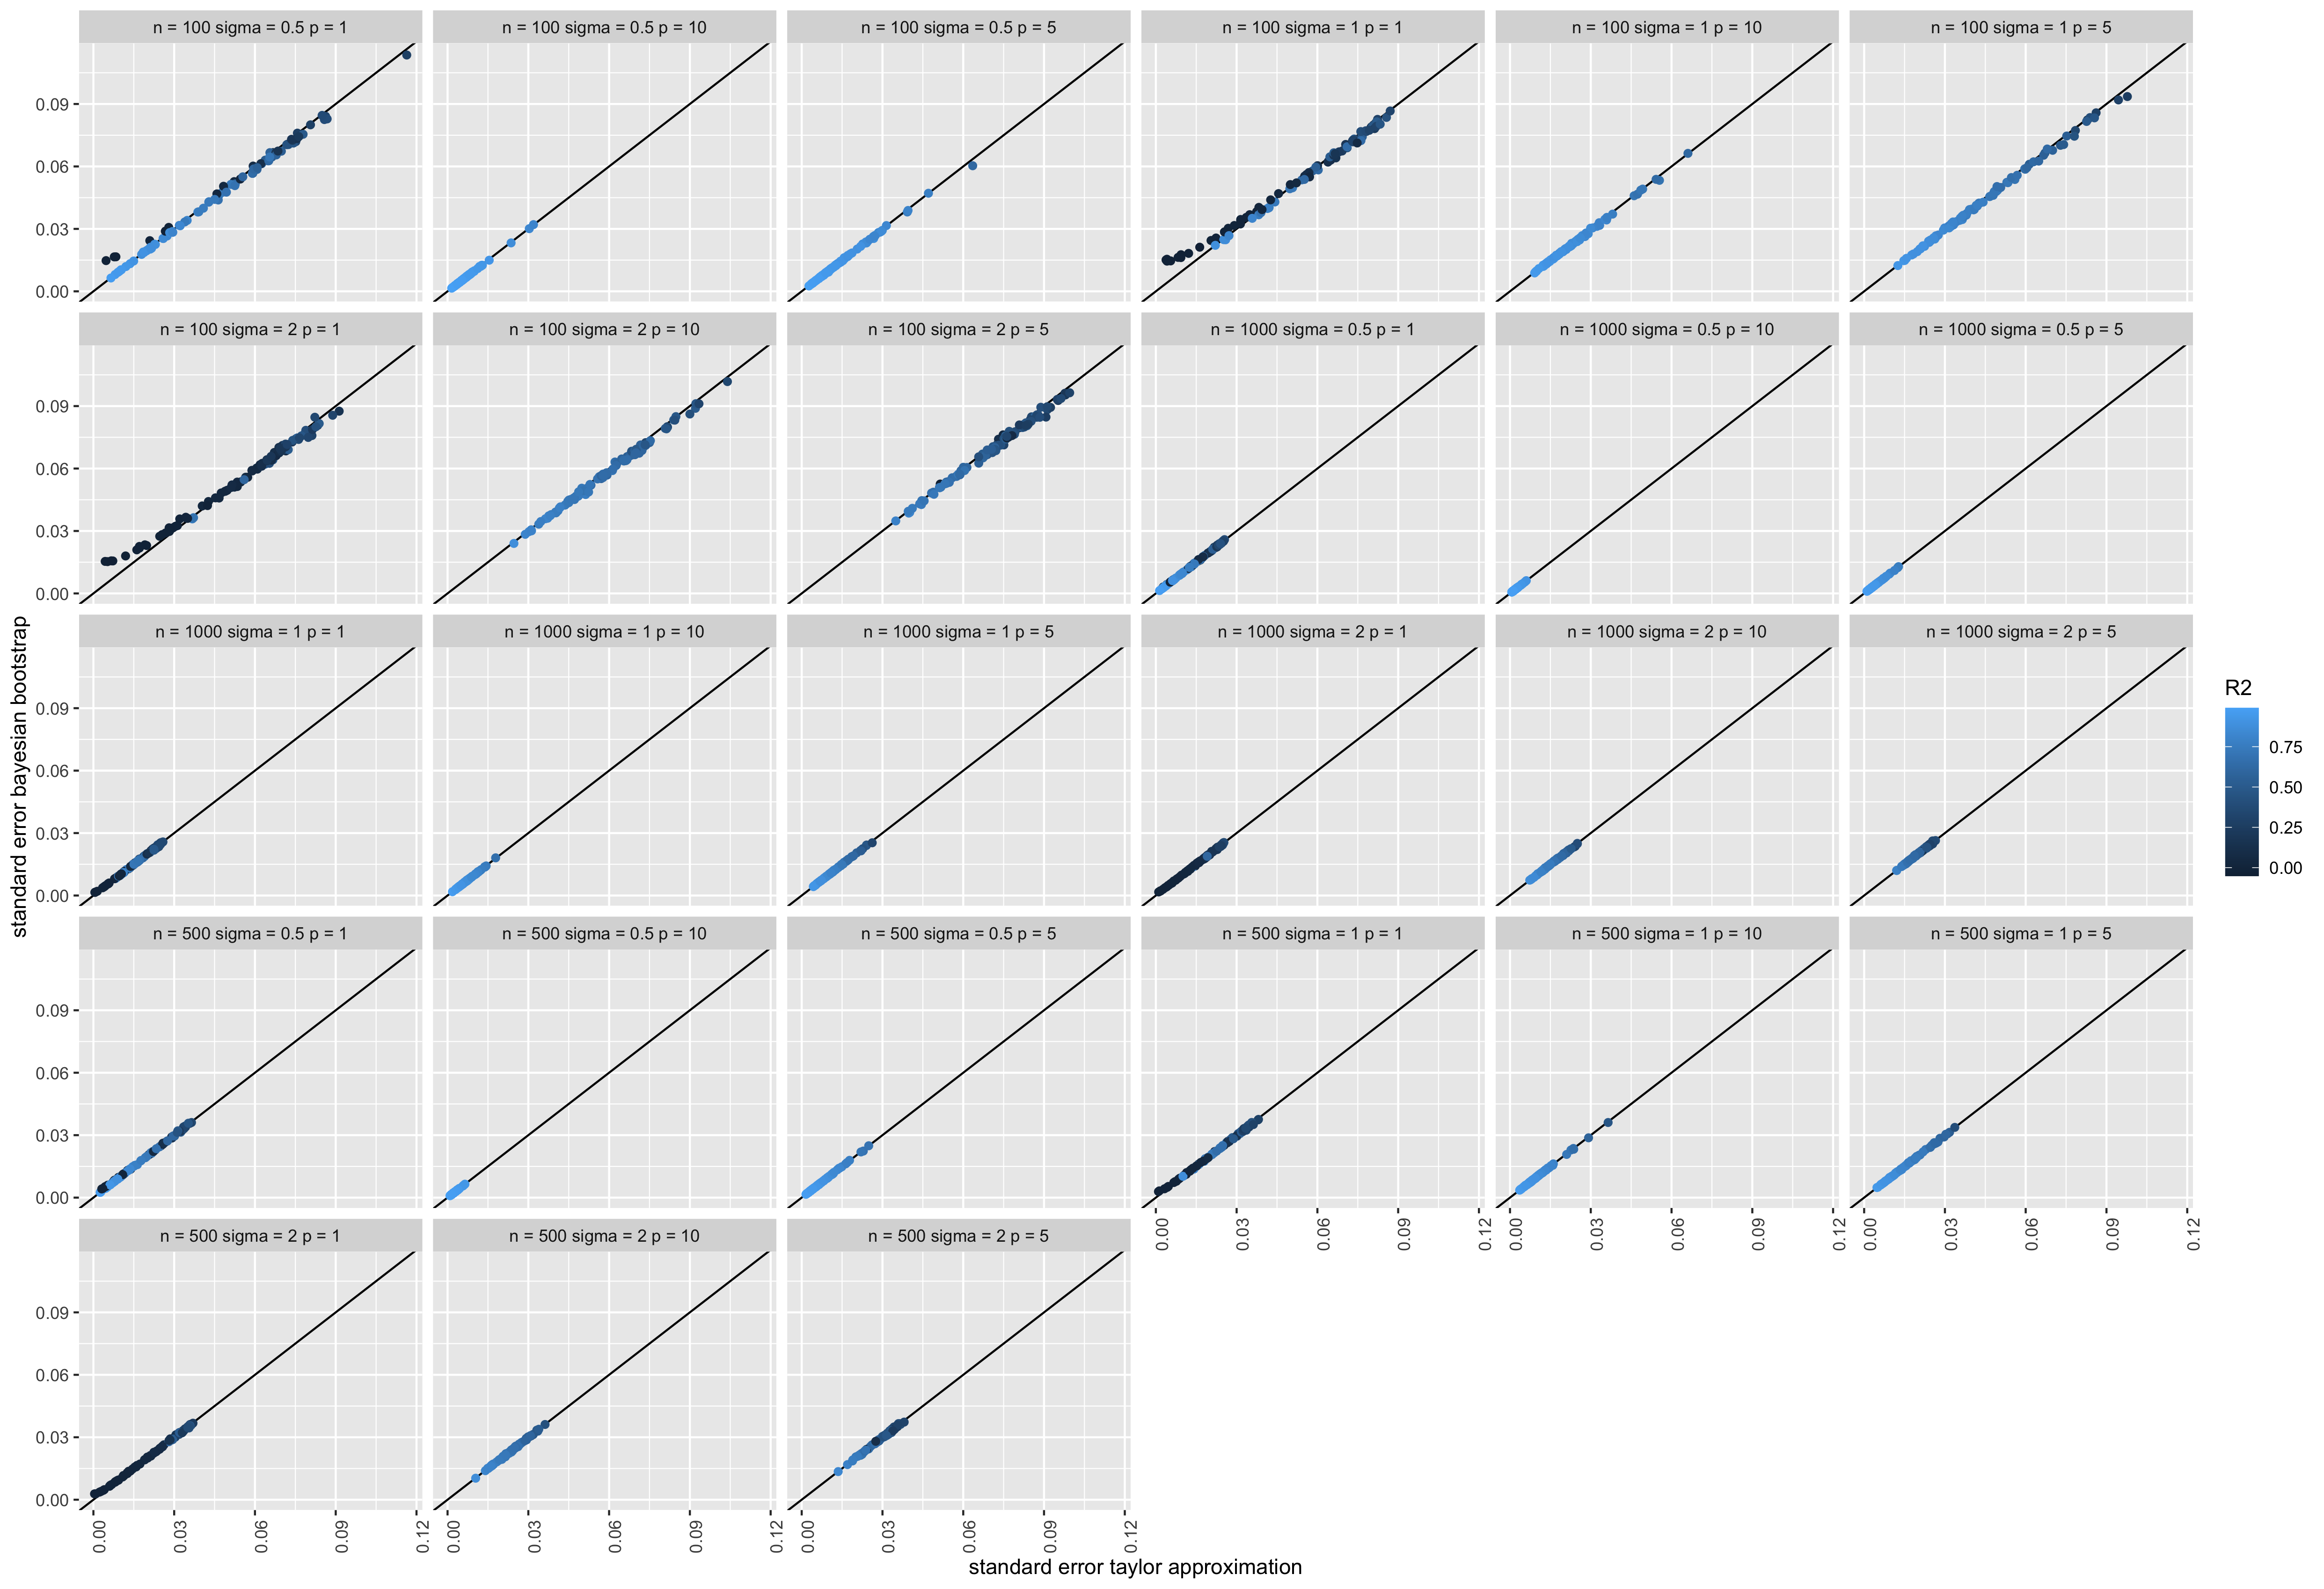
\includegraphics[width=\textwidth]{simres.png}
    \caption{ Simulation results for larger values of n}
    \label{fig:simres}
\end{figure}

Figure \ref{fig:simres_low_n} runs similar experiments, but $n$ is now either 5 or 10. Not surprisingly, we see more dispersion in the standard error estimates. One pattern seems to be that when the R2 estimate is small (darker dots) compared to the standard error, we start to bias in the Taylor approximation.

\begin{figure}
    \centering
    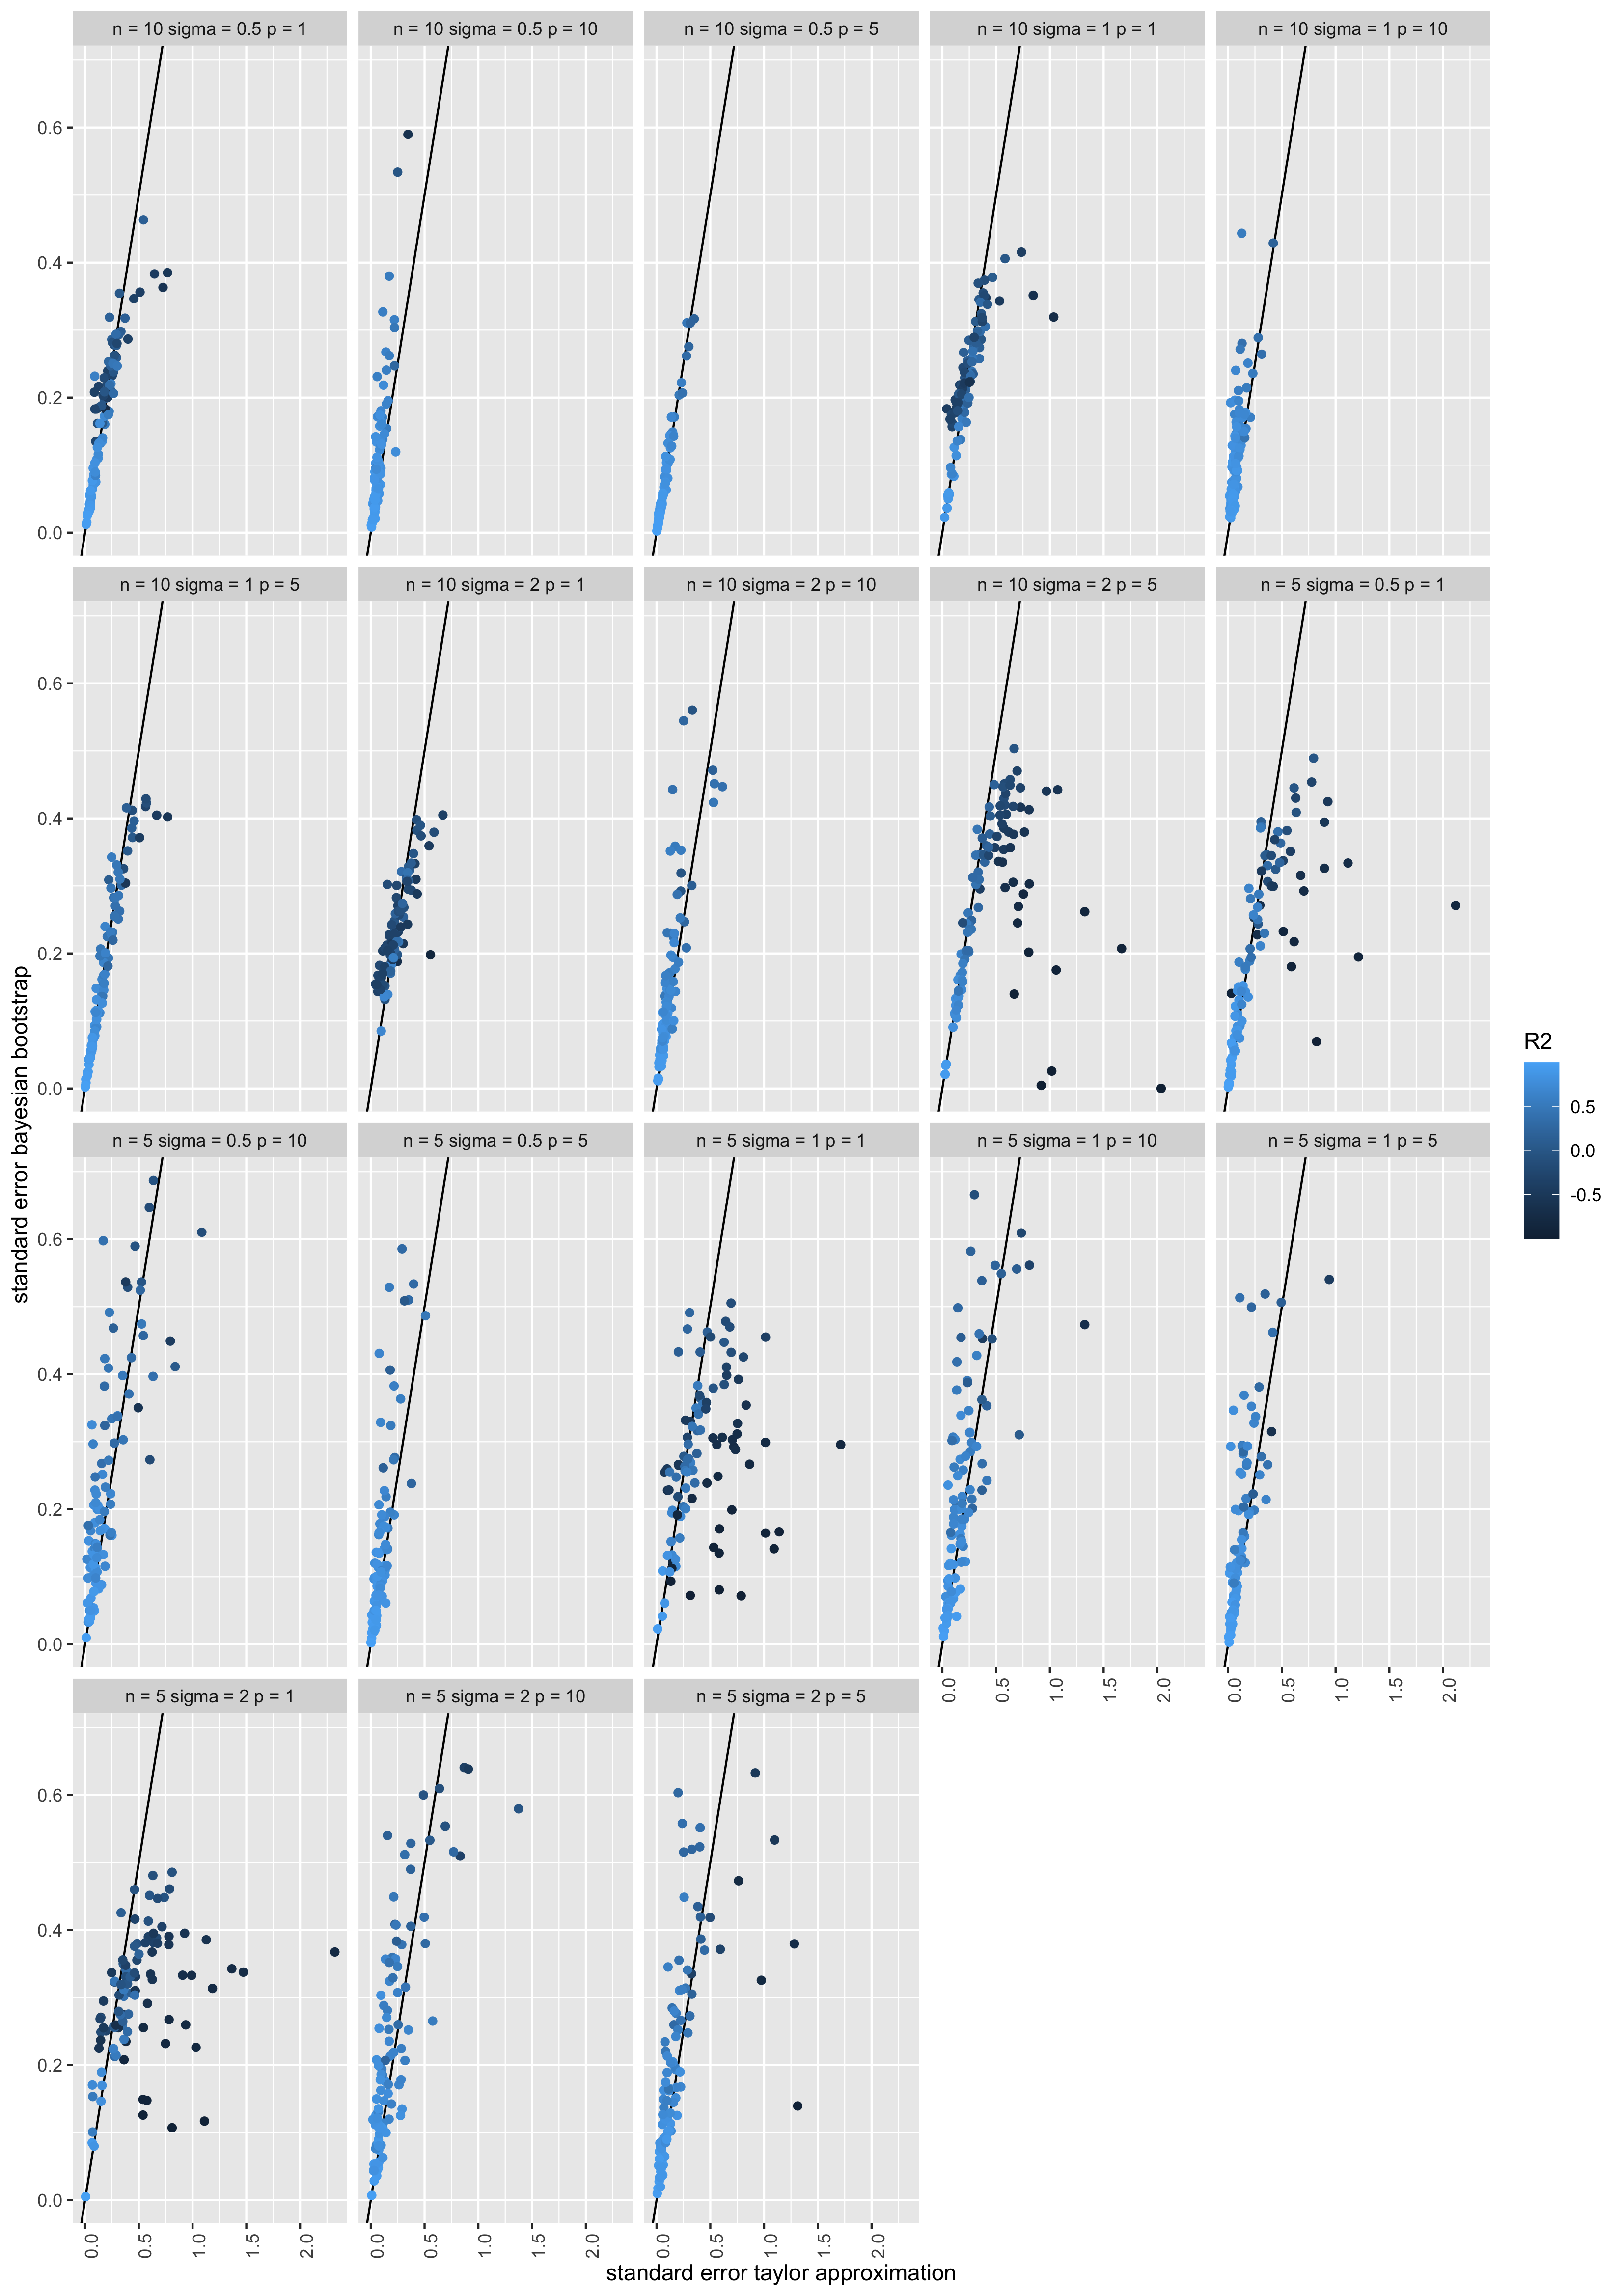
\includegraphics[width=\textwidth]{simres_low_n.png}
    \caption{ Simulation results for lower values of n}
    \label{fig:simres_low_n}
\end{figure}


\newpage
\bibliographystyle{plainnat}
\bibliography{references.bib}

\end{document}